\documentclass[aspectratio=169]{beamer}
\usetheme{simple}

\input{preamble/preamble.tex}
\input{preamble/preamble_math.tex}
% \input{preamble/preamble_acronyms.tex}

\title{Transformers}
\subtitle{STATS305B: Applied  Statistics II}
\author{Scott Linderman}
\date{\today}


\begin{document}


\maketitle

\begin{frame}{Last Time...}
    \begin{itemize}
        \item (Probabilistic) PCA as a (stochastic) linear autoencoder
        \item Variational Autoencoders (VAEs)
        \item Review of Gradient-based Variational Inference
        \item Demo
    \end{itemize}
    \vspace{1em}
\end{frame}

\begin{frame}{Today...}
    \textbf{Outline:}
    \begin{itemize}
        \item Transformers
        \item Self-Attention
        \item MLPs
        \item Other Tricks
    \end{itemize}
    \vspace{1em}
\end{frame}

    
\begin{frame}[t,allowframebreaks]{Transformers}\label{transformers}
    
Transformers are deep neural networks that underly modern large
language models like ChatGPT, Gemini, and Claude. 

They are also widely used for computer vision tasks by treating each 
patch of an image as a "token."

The basic building blocks of a transformer include: self-attention,
token-wise nonlinear transformations, layer norm, and positional
encodings. 

We will focus on modeling sequential data. We will follow the
presentation of Turner et al. (2023), but we will
make some slight modifications to the notation to be consistent with
Homework 4.
\end{frame}

\begin{frame}[t,allowframebreaks]{Preliminaries}\label{preliminaries}

Let \(\mbX^{(0)} \in \reals^{T \times D}\) denote our data matrix with
row \(\mbx_t^{(0)} \in \reals^D\) representing the \(t\)-th
\textbf{token} in the sequence. For example, the tokens could be a
vector embedding of a word, sub-word, or character. The embeddings may
be fixed or learned as part of the model.

The output of the transformer will be another matrix of the same shape,
\(\mbX^{(M)} \in \reals^{T \times D}\). These output features can be
used for downstream tasks like sentiment classification, machine
translation, or autoregressive modeling.

The output results from a stack of transformer blocks, 
\begin{align*}
\mbX^{(m)} &= \texttt{transformer-block}(\mbX^{(m-1)})
\end{align*} 

Each block consists of two stages: one that operates
vertically, combining information across the sequence length; another
that operates horizontally, combining information across feature
dimensions.

\begin{figure}
\centering
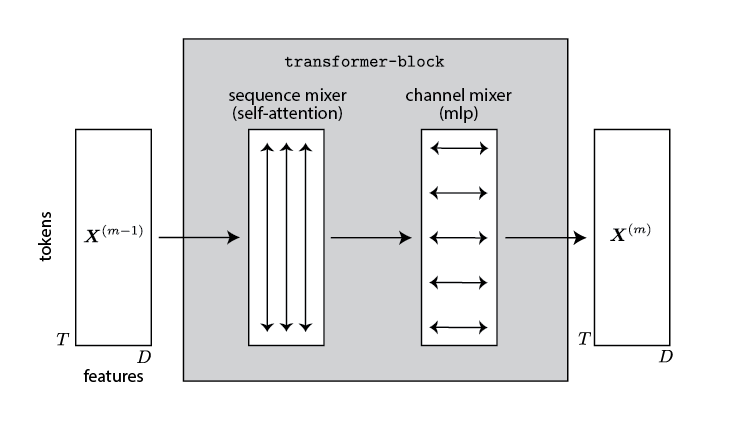
\includegraphics[width=.7\textwidth]{../lectures/figures/14_transformers/transformer-block.png}
\caption{Transformer Block}
\end{figure}
\end{frame}

\begin{frame}[t,allowframebreaks]{Attention}\label{attention}

The first stage combines information across sequence length using a
mechanism called \textbf{attention}. 

Mathematically, attention is just a
weighted average, 
\begin{align*}
\mbY^{(m)} &= \mbA^{(m)} \mbX^{(m-1)},
\end{align*} 
where \(\mbA^{(m)} \in \reals_+^{T \times T}\) is a
row-stochastic attention matrix. 

That is, \(\sum_{s} A_{ts}^{(m)} = 1\)
for all \(t\). 

Intuitively, \(A_{t,s}^{(m)}\) indicates how much output
location \(t\) attends to input location \(s\).
\begin{figure}
    \centering
    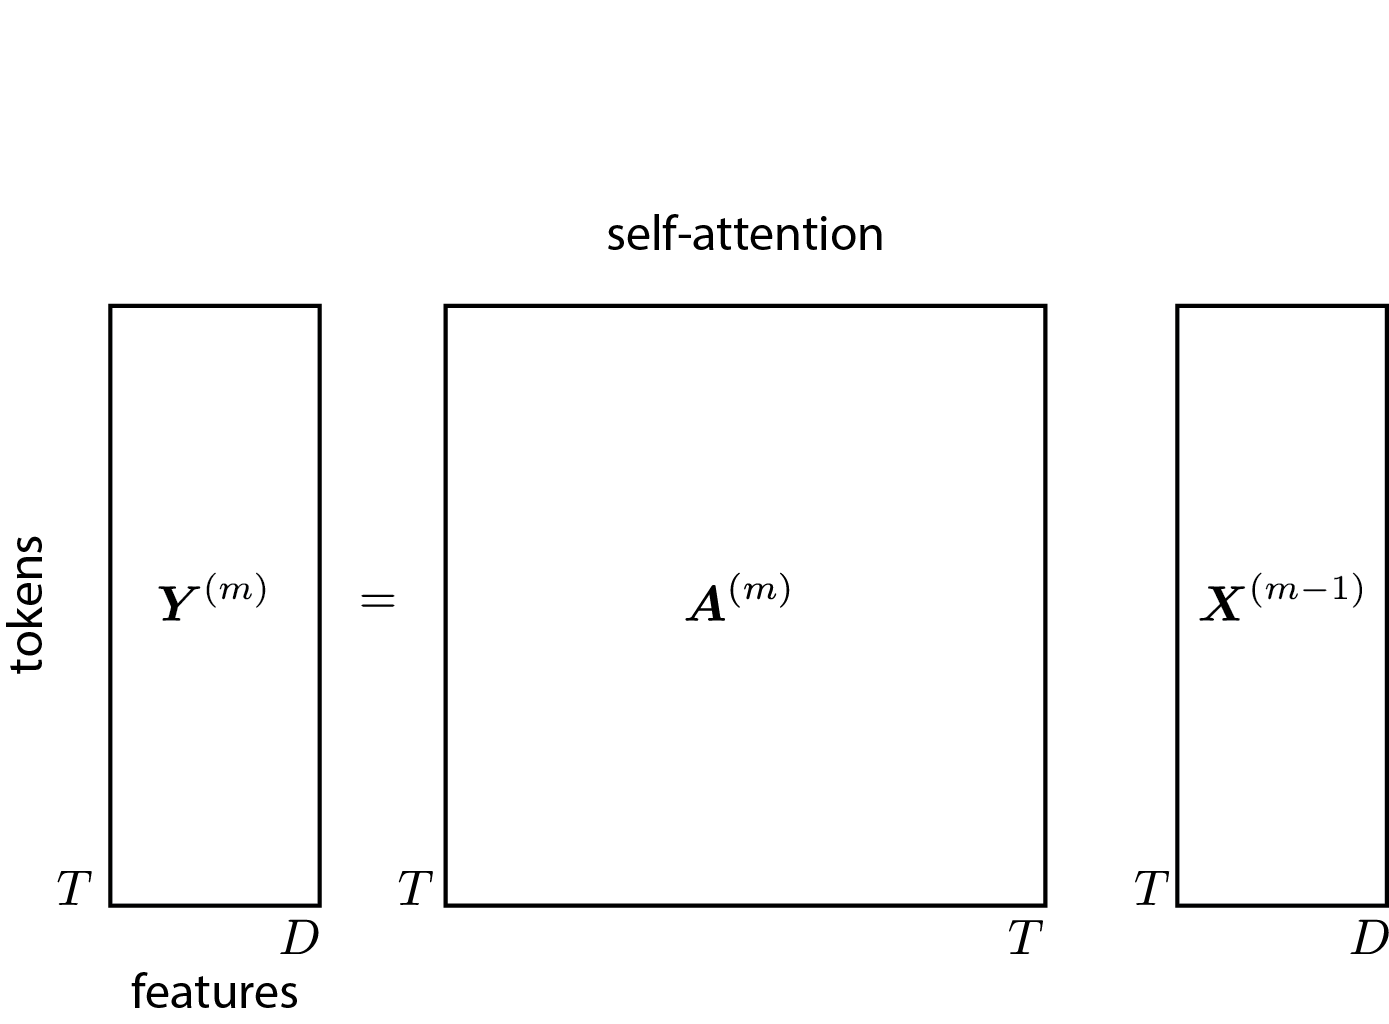
\includegraphics[width=.55\textwidth]{../lectures/figures/14_transformers/self-attention-1.png}
    \caption{Self Attention}
\end{figure}
\end{frame}

\begin{frame}[t,allowframebreaks]{Self-Attention}\label{self-attention}

Where does the attention matrix come from? In a transformer, the
attention weights are determined by the pairwise similarity of tokens in
the sequence. 

The simplest instantiation of this idea would be something like, 
\begin{align*}
A_{t,s} &\propto \exp \left\{ \mbx_t^\top \mbx_s \right\}
\end{align*} 

Once normalized, 
\begin{align*}
A_{t,s} &= \frac{\exp \{ \mbx_t^\top \mbx_s\}}{\sum_{s'=1}^T \exp\{\mbx_t^\top \mbx_{s'}\}}.
\end{align*} 

(Note: we have dropped the superscript \({}^{(m)}\) for
clarity in this section.)

This approach implies that attention depends equally on all \(D\)
dimensions of the embedding, but some dimensions may
convey different kinds of information that may be of greater or lesser
relevance for the attention mechanism. 

One way to allow for this is to
project the tokens into a feature space before computing the attention
weights, 
\begin{align*}
A_{t,s} &= \frac{\exp \{ (\mbU \mbx_t)^\top (\mbU \mbx_s)\}}{\sum_{s'=1}^T \exp\{(\mbU \mbx_t)^\top (\mbU \mbx_{s'}) \}}
\end{align*} 
where \(\mbU \in \reals^{K \times D}\) with \(K < D\).

If the attention weight specifies how relevant token \(\mbx_s\) is
to updating the feature representation for token \(\mbx_t\), then
directionality may matter. Transformers address this asymmetry with,
\begin{align*}
A_{t,s} &= \frac{\exp \{ (\mbU_q \mbx_t)^\top (\mbU_k \mbx_s)\}}{\sum_{s'=1}^T \exp\{(\mbU_q \mbx_t)^\top (\mbU_k \mbx_{s'}) \}},
\end{align*} 
where \(\mbU_q \mbx_t \in \reals^{K}\) are the
\textbf{queries} and \(\mbU_k \mbx_s \in \reals^{K}\) are the
\textbf{keys}.

The parameters \(\mbU_q \in \reals^{K \times D}\) and
\(\mbU_k \in \reals^{K \times D}\) define the
self-attention mechanism.

\begin{figure}
\centering
{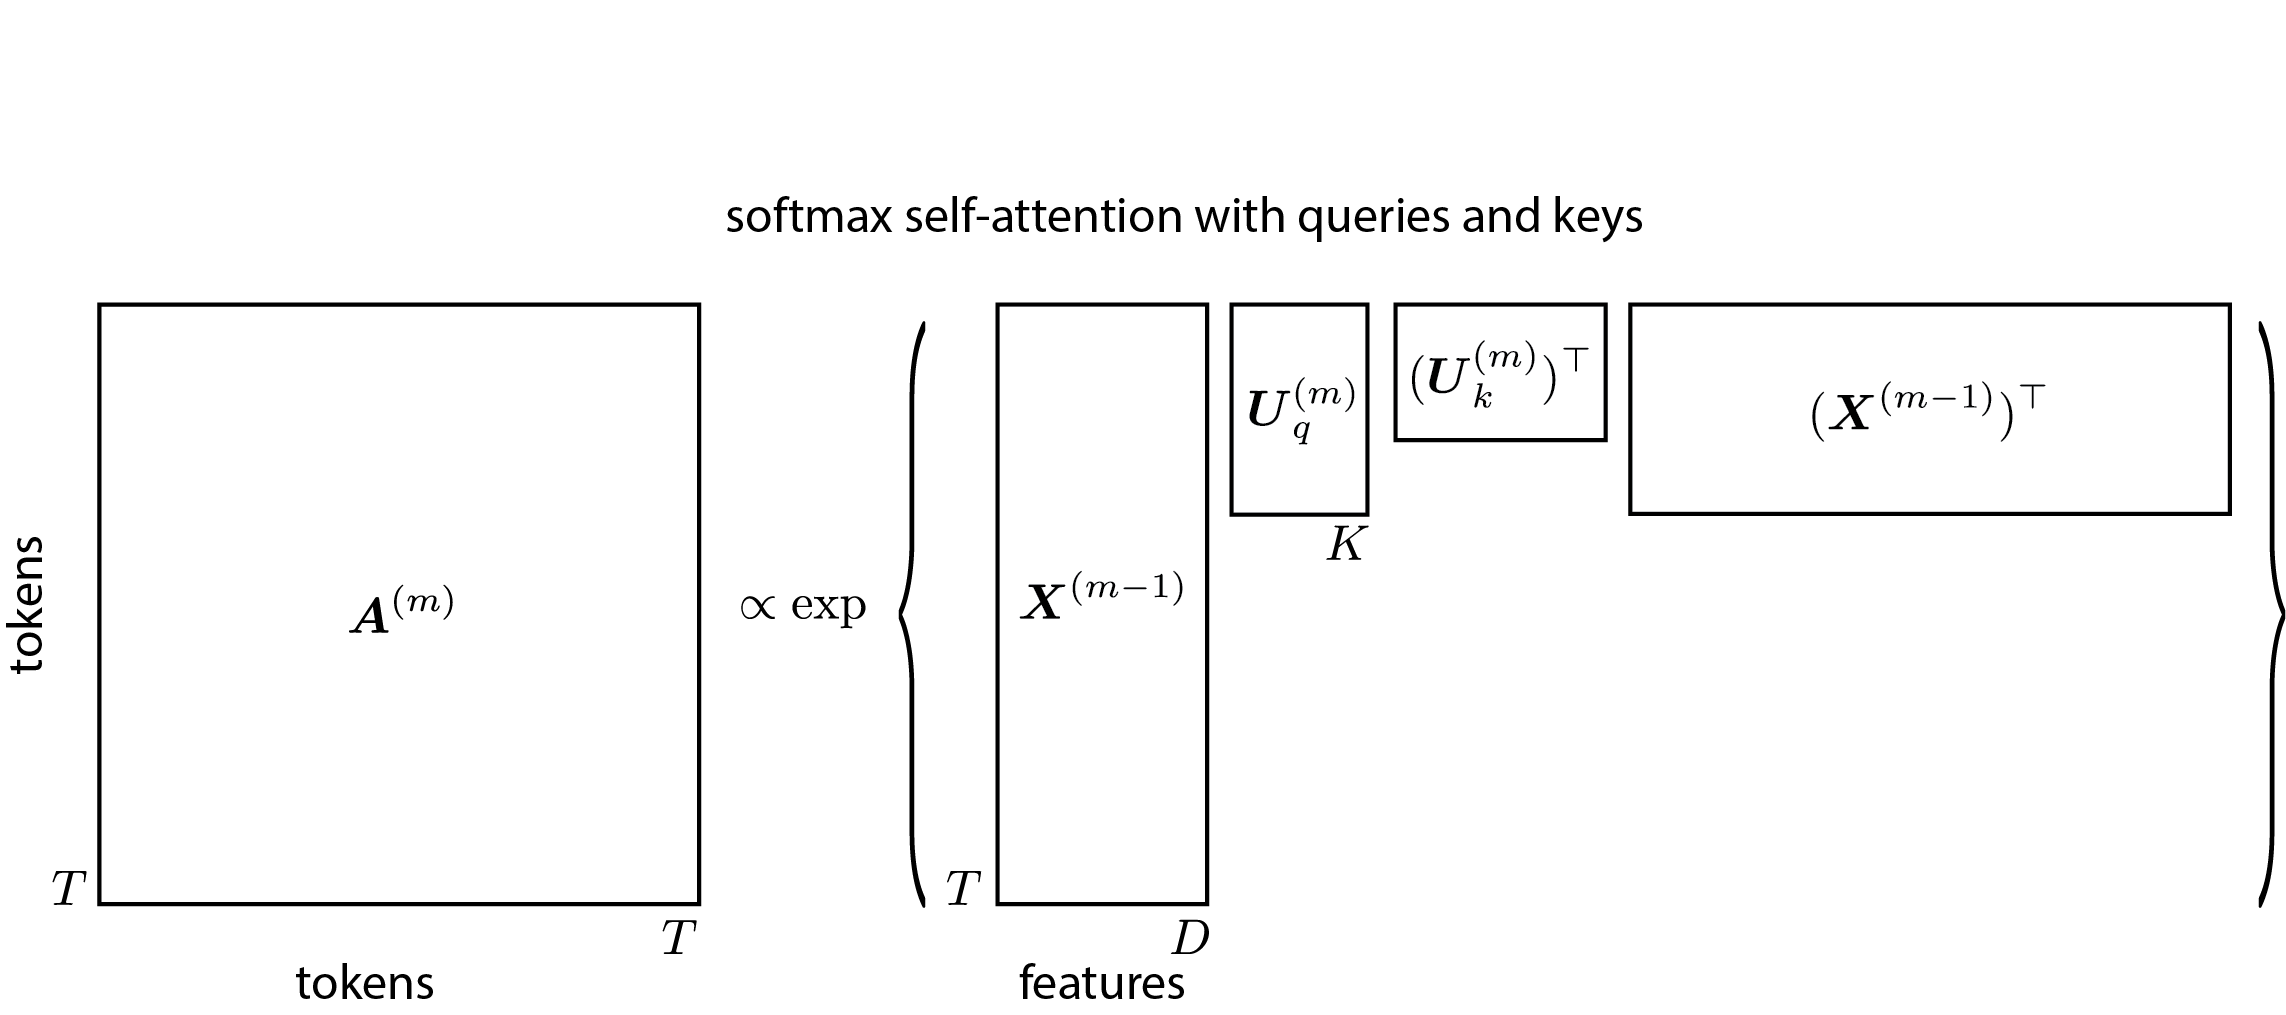
\includegraphics[width=.9\textwidth]{../lectures/figures/14_transformers/self-attention-2.png}}
\caption{Self Attention with Queries and Keys}
\end{figure}
\end{frame}

\begin{frame}[t,allowframebreaks]{Causal Self-Attention}

When we are using transformers for autoregressive sequence modeling, we
constrain the attention matrix to be \textbf{causal} by requiring
\(A_{t,s}^{(m)} = 0\) for all \(t < s\). 

In other words, the matrix is \textbf{lower triangular}.

To enforce this constraint, we simply mask the upper triangular part of the attention
matrix and normalize the rows appropriately, 
\begin{align*}
A_{t,s} &= \frac{\exp \{ (\mbU_q \mbx_t)^\top (\mbU_k \mbx_s)\}}{\textcolor{red}{\sum_{s'=1}^{t}} \exp\{(\mbU_q \mbx_t)^\top (\mbU_k \mbx_{s'})\}} \cdot \bbI[t \geq s].
\end{align*}
\end{frame}

\begin{frame}[t,allowframebreaks]{Comparison to RNNs }
Compare the self-attention mechanism to the information processing in an RNN. 

Rather than propagating information about past tokens via a hidden state, a
transformer with causal attention can directly attend to any one of the
past tokens.
\end{frame}

\begin{frame}[t,allowframebreaks]{Comparison to Convolutional Neural Networks (CNNs)}
If the attention weights were only a function of the distance between
tokens, \(A_{t,s} = a_{t-s}\), then the matrix \(\mbA\) would be a
\textbf{Toeplitz matrix}. 

Multiplication by a Toeplitz matrix corresponds to a discrete convolution. 

From this perspective, we can think of the attention mechanism in a transformer 
as a generalization of convolution that allows for input-dependent and 
time-varying filters.
\end{frame}

\begin{frame}[t,allowframebreaks]{Multi-Headed Self-Attention}\label{multi-headed-self-attention}

Just as in a CNN each layer performs convolutions with a bank of filters
in parallel, in a transformer each block uses a bank of \(H\)
\textbf{attention heads} in parallel. 

Let, 
\begin{align*}
\mbY^{(m,h)} &= \mbA^{(m,h)} \mbX^{(m-1)} \in \reals^{T \times D}
\end{align*} 
where 
\begin{align*}
A_{t,s}^{(m,h)} &= 
\frac{\exp \{ (\mbU_q^{(m,h)} \mbx_t^{(m-1)})^\top (\mbU_k^{(m,h)} \mbx_s^{(m-1)})\}}{\sum_{s'=1}^T \exp\{(\mbU_q^{(m,h)} \mbx_t^{(m-1)})^\top (\mbU_k^{(m,h)} \mbx_{s'}^{(m-1)}) \}},
\end{align*} 
is an attention weight at layer \(m\) and head \(h\) for
\(h=1,\ldots,H\). 

(Now you see why we dropped superscripts above --- the
notation is a handful!)

\begin{figure}
\centering
{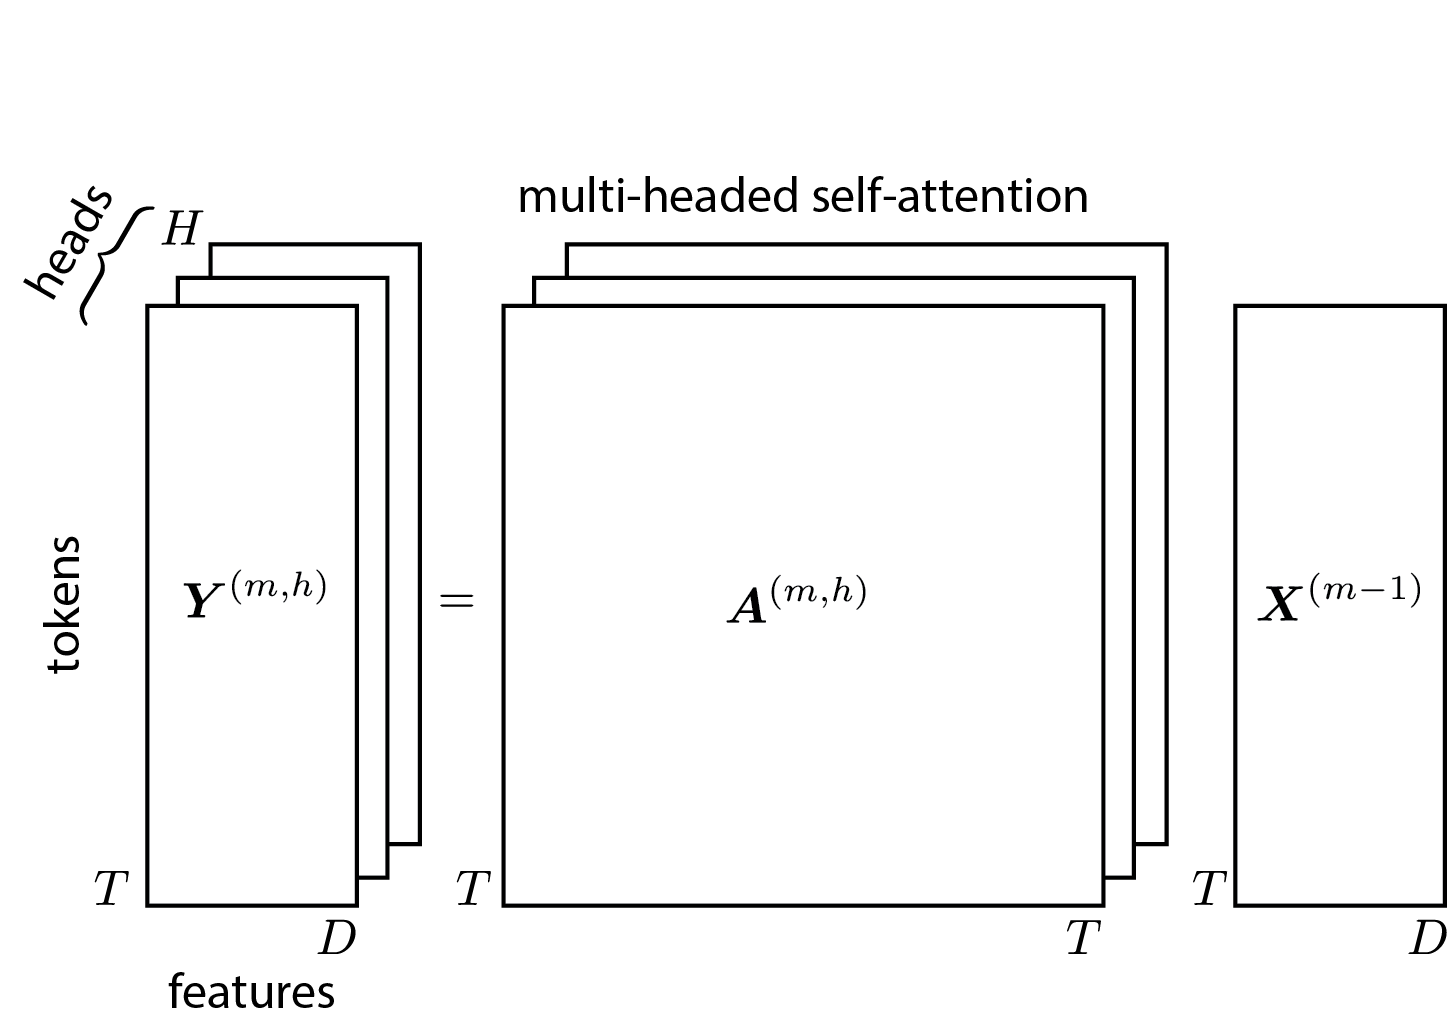
\includegraphics[width=.7\textwidth]{../lectures/figures/14_transformers/mhsa-1.png}}
\caption{Multi-Headed Self Attention}
\end{figure}

The outputs of the attention heads are either concatenated or linearly
combined, \begin{align*}
\mbY^{(m)} &= \sum_{h=1}^H \mbY^{(m,h)} (\mbV^{(m,h)})^\top \\
&\triangleq \texttt{mhsa}(\mbX^{(m-1)}).
\end{align*} where \(\mbV^{(m,h)} \in \reals^{D \times D}\) is a
read-out matrix for layer \(m\), head \(h\). We denote the multi-headed
self-attention (MHSA) mapping by \(\texttt{mhsa}(\cdot)\).

\begin{figure}
\centering
{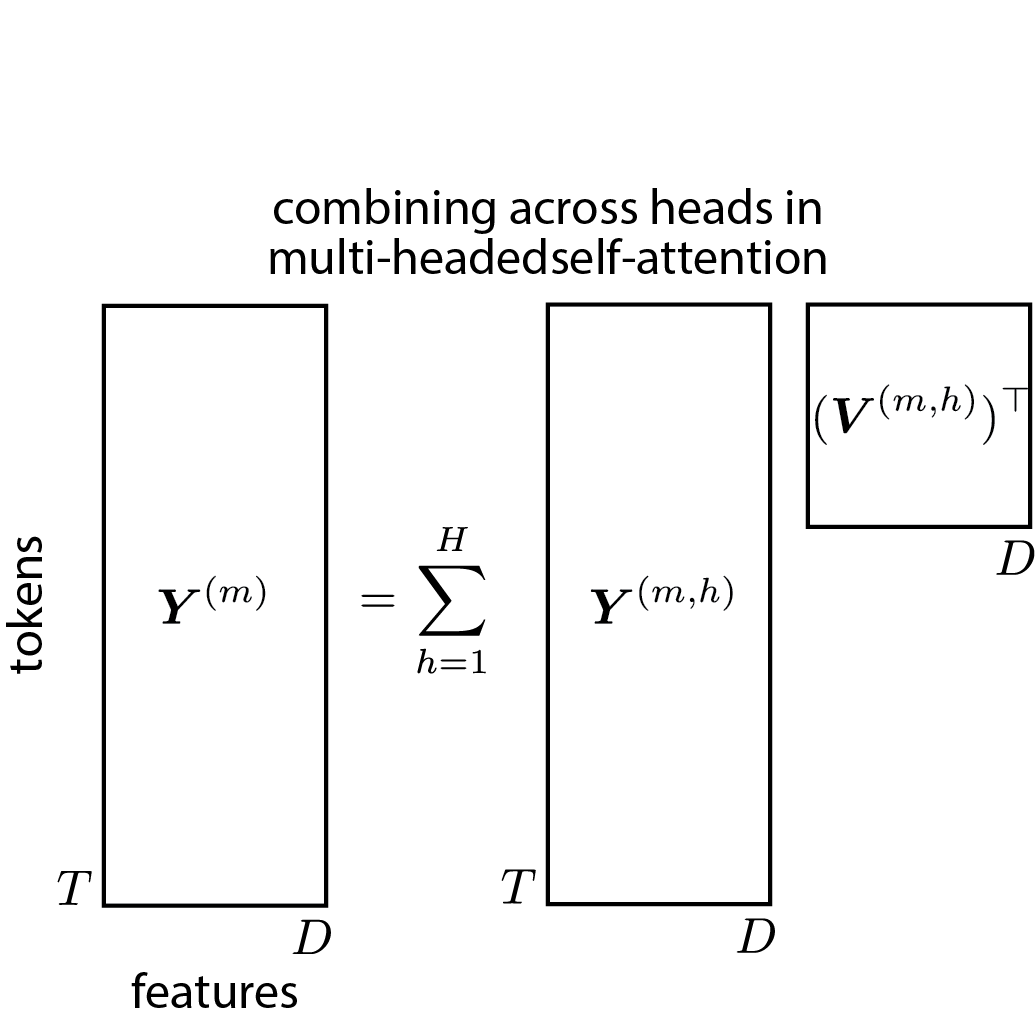
\includegraphics[width=.7\textwidth]{../lectures/figures/14_transformers/mhsa-2.png}}
\caption{Multi-Headed Self Attention}
\end{figure}
\end{frame}

\begin{frame}[t,allowframebreaks]{Queries, Keys, and Values}\label{queries-keys-and-values}
The original transformer paper presents the output of a single head as a 
set of values,
\begin{align*}
\mbY^{(m,h)} &= \mbA^{(m,h)} (\mbX^{(m-1)} (\mbU_v^{(m,h)})^\top) \in \reals^{T \times K}
\end{align*} 
where \(\mbU_v^{(m,h)} \in \reals^{K \times D}\) is a
\textbf{value matrix}. 

Then the attention mechanism can be though of as
taking a weighted average of \textbf{values} \(\mbU_v \mbx_t\) where the
weights are determined by an inner product between the queries and keys.

The final output is projected back into the original token dimension and
linearly combined, 
\begin{align*}
\mbY^{(m)} &= \sum_{h=1}^H \mbY^{(m,h)} (\mbU_o^{(m,h)})^\top 
\end{align*} 
where \(\mbU_o^{(m,h)} \in \reals^{D \times K}\) is an
\textbf{output matrix} that maps from values to new tokens.

This formulation corresponds to a low-rank read-out matrix
\(\mbV = \mbU_o \mbU_v^\top\), where we have again dropped the
superscripts for clarity. 
\end{frame}

\begin{frame}[t,allowframebreaks]{Token-wise Nonlinearity}\label{token-wise-nonlinearity}

After applying the multi-headed self-attention to obtain \(\mbY^{(m)}\),
the transformer applies a token-wise nonlinear transformation to
nonlinearly mix the feature dimensions. 

This is done with a simple feedforward neural network, also known as a \textbf{multilayer
perceptron (MLP)}, \begin{align*}
\mbx_t^{(m)} &= \texttt{mlp}(\mby_t^{(m)})
\end{align*} Note that the same function is applied to all positions
\(t\).

\begin{figure}
\centering
{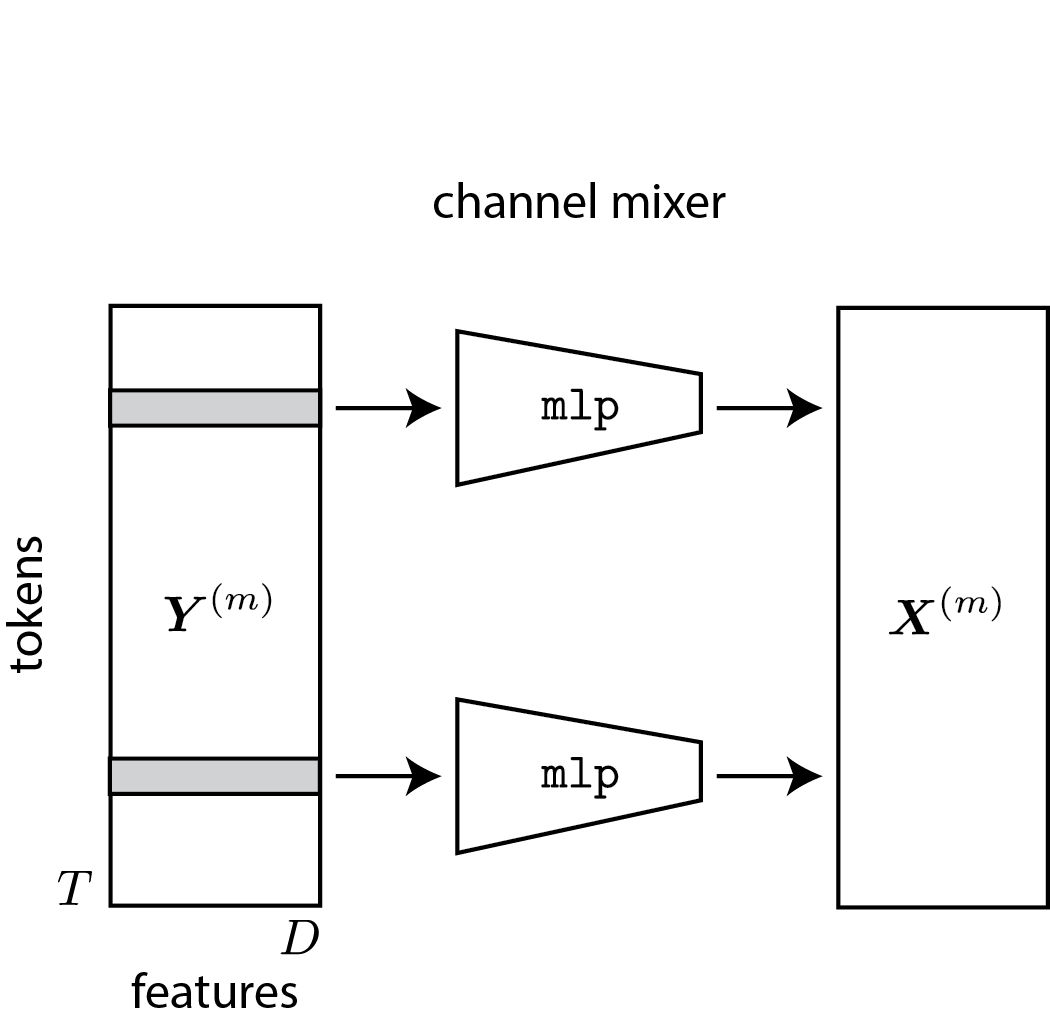
\includegraphics[width=.4\textwidth]{../lectures/figures/14_transformers/mlp.png}}
\caption{MLP}
\end{figure}
\end{frame}

\begin{frame}[t,allowframebreaks]{Computational Complexity}\label{computational-complexity}
The cost of self-attention is $\cO(T^2K)$. It scales quadratically with the sequence length  
(or more specifically, the length of the context window).

The MLP typically has hidden dimensions of at least \(D\), so the computational
complexity of this step is at least \(\cO(TD^2)\). 

For transformers with very
large featured dimensions, the MLP can be the dominant cost. 
\end{frame}

\begin{frame}[t,allowframebreaks]{Residual Connections}\label{residual-connections}

Rather than parameterizing \(\mbX^{(m)}\) as the output of the MLP, a
common trick in deep learning is to use residual connections. 

Simple idea: when the input and output are of the same dimensionality, we
can let the network learn the \textbf{residual}, which is typically
smaller in magnitude than the overall function.

Transformers use residual connections for both the multi-headed
self-attention step and the MLP. So, \begin{align*}
\mbY^{(m)} &= \mbX^{(m-1)} + \texttt{mhsa}(\mbX^{(m-1)}) \\
\mbX^{(m)} &= \mbY^{(m)} + \texttt{mlp}(\mbY^{(m)})
\end{align*}

\begin{figure}
\centering
{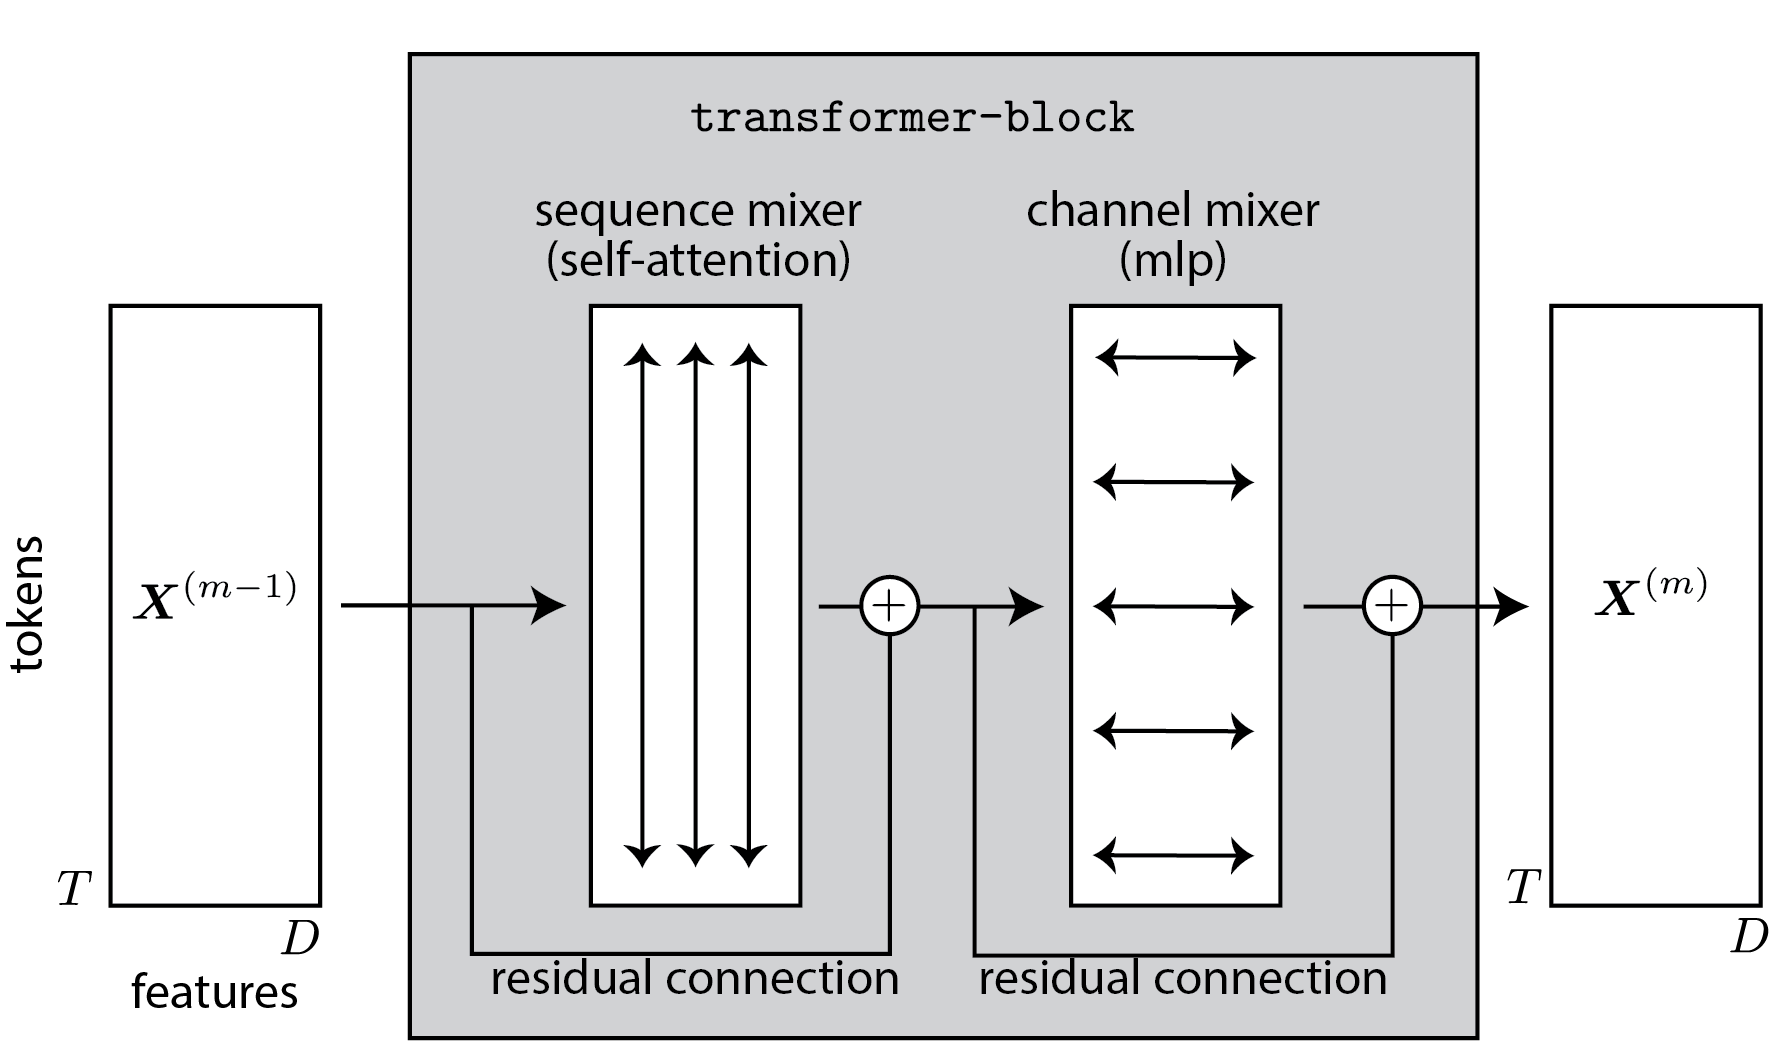
\includegraphics[width=.7\textwidth]{../lectures/figures/14_transformers/residual-conn.png}}
\caption{Residual Connections}
\end{figure}
\end{frame}

\begin{frame}[t,allowframebreaks]{Layer Norm}\label{layer-norm}

Finally, it is important to use other deep learning ``tricks'' like
LayerNorm to stabilize training. 
In a transformer, LayerNorm amounts to
z-scoring each token \(\mbx_t\) and then shifting and scaling each
feature dimension, 
\begin{align*}
\texttt{layer-norm}(\mbx_t) 
&= \mbbeta + \mbgamma \odot \left( \frac{\mbx_t - \texttt{mean}(\mbx_t)}{\texttt{std}(\mbx_t)} \right)
\end{align*} 
where 
\begin{align*}
\texttt{mean}(\mbx_t) &= \frac{1}{D} \sum_{d=1}^D x_{t,d} \\
\texttt{std}(\mbx_t) &= \Big(\frac{1}{D} \sum_{d=1}^D (x_{t,d} - \texttt{mean}(\mbx_t))^2 \Big)^{\frac{1}{2}}
\end{align*} 
and $\mbbeta, \mbgamma \in \reals^D$ are learned parameters.

LayerNorm is typically applied before the multi-headed self-attention
and MLP steps, 
\begin{align*}
\overline{\mbX}^{(m-1)} &= \texttt{layer-norm}(\mbX^{(m-1)}) \\
\mbY^{(m)} &= \overline{\mbX}^{(m-1)} + \texttt{mhsa}(\overline{\mbX}^{(m-1)}) \\
\overline{\mbY}^{(m)} &= \texttt{layer-norm}(\mbY^{(m)}) \\
\mbX^{(m)} &= \overline{\mbY}^{(m)} + \texttt{mlp}(\overline{\mbY}^{(m)})
\end{align*} 
This defines one \(\texttt{transformer-block}\).

A transformer stacks \(M\) \(\texttt{transformer-blocks}\) on top of one
another to produce a deep sequence-to-sequence model.
\end{frame}

\begin{frame}[t,allowframebreaks]{Positional Encodings}\label{positional-encodings}

Except for the lower triangular constraint on the attention matrices,
the transformer architecture knows nothing about the relative positions
of the tokens. 

Absent this constraint, the transformer essentially
treats the data as an \textbf{unordered set} of tokens. 

This can actually be a feature! It allows the transformer to act on a wide range
of datasets aside from just sequences. 

However, when the data posses some spatial or temporal structure, it is
helpful to include that information in the embedding. A simple way to do
so is to add position and content in the token, 
\begin{align*}
\mbx_t^{(0)} &= \mbc_t + \mbp_t,
\end{align*} 
where \(\mbc_t \in \reals^D\) is an embedding of the content and \(\mbp_t \in \reals^D\) encodes the position (e.g., with a
set of sinusoidal basis functions).
\end{frame}

\begin{frame}[t,allowframebreaks]{Autoregressive Modeling}\label{autoregressive-modeling}

To use a transformer for autoregressive modeling, we need to make
predictions from the final layer's representations. 

If the goal is to predict the next word label \(\ell_{t+1} \in \{1,\ldots,V\}\) 
based on encodings of past words \(\mbx_{1:t}^{(0)}\), where \(V\) is the
vocabulary size, then we could use a categorical distribution,
\begin{align*}
\ell_{t+1} &\sim \mathrm{Cat}(\mathrm{softmax}(\mbW \mbx_t^{(M)}))
\end{align*} 
where \(\mbW \in \reals^{V \times D}\). 

Like the hidden states in an RNN, the final layer's representations \(\mbx_t^{(M)}\)
combine information from all tokens up to and including index \(t\).
\end{frame}

\begin{frame}[t,allowframebreaks]{Training}\label{training}

Training deep neural networks is somewhat of a dark art. 

Standard practice is to use the Adam optimizer with a bag of tricks including
gradient clipping, learning rate annealing schedules, increasing
minibatch sizes, dropout, etc. 

Generally, treat these algorithmic decisions as hyperparameters to be tuned. 

We won't try to put any details in writing lest you overfit to them.
\end{frame}

\begin{frame}[t,allowframebreaks]{Conclusion}\label{conclusion}

Transformers are a workhorse of modern machine learning and key to many
of the impressive advances over recent years. 

However, there are still areas for improvement. For example, the computational cost of attention
is \(\cO(T^2)\), and a lot of work has gone into cutting that down.

Likewise, while the transformer allows for predictions to be made in
parallel across an entire sequence, sampling from the learned
autoregressive model is still takes linear time. 

In the lectures ahead, we'll discuss other recent architectures that 
address some of these concerns.
\end{frame}

    
\end{document}
